%----------------------------------------------------------------------------------------
%	PACKAGES AND OTHER DOCUMENT CONFIGURATIONS
%----------------------------------------------------------------------------------------
\documentclass{memoir}
\usepackage[utf8]{inputenc}
\usepackage{titlesec}
\usepackage{lmodern}
\usepackage[T1]{fontenc}
\usepackage{float}
\usepackage{fancyhdr} % Required for custom headers
\usepackage{lastpage} % Required to determine the last page for the footer
\usepackage{extramarks} % Required for headers and footers
\usepackage[usenames,dvipsnames]{color} % Required for custom colors
\usepackage{graphicx} % Required to insert images
\usepackage{listings} % Required for insertion of code
\usepackage{courier} % Required for the courier font
\usepackage{lipsum} % Used for inserting dummy 'Lorem ipsum' text into the template
\usepackage[section]{placeins} %when placing img
\usepackage{url}
\usepackage{hyperref}
\usepackage[table,xcdraw]{xcolor}


% Margins
\topmargin=-.45in
\evensidemargin=0in
\oddsidemargin=0in
\textwidth=6.5in
\textheight=9.0in
\headsep=0.25in
\linespread{1.1} % Line spacing

\hypersetup{
    colorlinks,
    linktoc = all,
    citecolor=black,
    filecolor=black,
    linkcolor=black,
    urlcolor=black
}
%----------------------------------------------------------------------------------------
%	DOCUMENT STRUCTURE COMMANDS
%	Skip this unless you know what you're doing
%----------------------------------------------------------------------------------------
\chapterstyle{culver}
\setsecnumdepth{subsubsection}
\renewcommand*\thesection{\arabic{section}}
\renewcommand*{\chapnumfont}{\huge\bfseries}
\renewcommand*{\chaptitlefont}{\huge\bfseries}
\renewcommand{\thefigure}{\arabic{chapter}.\arabic{figure}}
\renewcommand{\thetable}{\arabic{chapter}.\arabic{figure}}

\makepagestyle{DTU}							
\makepsmarks{DTU}{%
	\createmark{chapter}{left}{shownumber}{}{. \ }
	\createmark{section}{right}{shownumber}{}{. \ }
	\createplainmark{toc}{both}{\contentsname}
	\createplainmark{lof}{both}{\listfigurename}
	\createplainmark{lot}{both}{\listtablename}
	\createplainmark{bib}{both}{\bibname}
	\createplainmark{index}{both}{\indexname}
	\createplainmark{glossary}{both}{\glossaryname}
}
\nouppercaseheads							% Ingen Caps oenskes
\makeevenhead{DTU}{\hmwkTitle}{}{\leftmark}				
\makeoddhead{DTU}{\hmwkTitle}{}{\leftmark}		
\makeevenfoot{DTU}{\hmwkClass}{\thepage}{\hmwkAuthorName}
\makeoddfoot{DTU}{\hmwkClass}{\thepage}{\hmwkAuthorName}	% Definerer ulige siders sidefod (\makeoddfoot{Navn}{Venstre}{Center}{Hoejre})
\makeheadrule{DTU}{\textwidth}{0.5pt}						% Tilfoejer en streg under sidehovedets indhold
\makefootrule{DTU}{\textwidth}{0.5pt}{1mm}					% Tilfoejer en streg under sidefodens indhold
\copypagestyle{DTUchap}{DTU}					% Sidehoved for kapitelsider defineres som standardsider, men med blank sidehoved
\makeoddhead{DTUchap}{}{}{}
\makeevenhead{DTUchap}{}{}{}
\makeheadrule{DTUchap}{\textwidth}{0pt}
\aliaspagestyle{chapter}{DTUchap}		% Den ny style vaelges til at gaelde for chapters	
\pagestyle{DTU}		
%----------------------------------------------------------------------------------------
%	NAME AND CLASS SECTION
%----------------------------------------------------------------------------------------

\newcommand{\hmwkTitle}{Project 1 - BMI survey} % Assignment title
\newcommand{\hmwkDueDate}{Tuesday,\ 03\ 13,\ 2018} % Due date
\newcommand{\hmwkClass}{Introduction to statistics \- 02402} % Course/class
\newcommand{\hmwkClassTime}{Department of Applied Mathematics and Computer Science} % Kursusansvarlig profession
\newcommand{\hmwkClassInstructor}{Nina Munkholt Jakobsen,} % Teacher/lecturer
\newcommand{\hmwkAuthorName}{Frederik Rander Andersen, s164146} % Your name

%----------------------------------------------------------------------------------------
%	TITLE PAGE
%----------------------------------------------------------------------------------------

\title{
\noindent\makebox[\linewidth]{\rule{\textwidth}{1pt}} 
\textmd{\huge \textbf{\hmwkClass \\ \hmwkTitle}}\\
\large\vspace{0.1in}\hmwkDueDate\\
\vspace{0.1in}\large{\textit{\hmwkClassInstructor\ \hmwkClassTime}}
\noindent\makebox[\linewidth]{\rule{\textwidth}{1pt}} 
\vspace{1in}
}

\author{\large\textbf{\hmwkAuthorName}}
\date{} % Insert date here if you want it to appear below your name


%----------------------------------------------------------------------------------------

\begin{document}
\begin{figure}
	\centering
	
\includegraphics[scale=0.15]{dtulogo.png}
\end{figure}

\begin{figure}[!b]
	
\includegraphics[scale=0.25]{dtufooter.png}
\end{figure}
\maketitle
\thispagestyle{empty}
%----------------------------------------------------------------------------------------
%	TABLE OF CONTENTS
%----------------------------------------------------------------------------------------

\newpage
\begin{KeepFromToc}
	\tableofcontents 
	\thispagestyle{empty}
\end{KeepFromToc}
\newpage

%----------------------------------------------------------------------------------------
%	INTRODUCTION & OVERVIEW
%----------------------------------------------------------------------------------------
% if you have an abstract and such then use: 
% pagenumbering{roman}
\pagenumbering{arabic}

\chapter[Descriptive analysis]{\\ Descriptive analysis} % first [] is what you want in the TOC and {} is chapter title 

\section{a) - Data description and introduction}
Body Mass Index or BMI is a formula to describe whether a person is overweight or not. It only considers height and weight, not things such as body fat. The formula is simply: 
$$ BMI = \frac{weight(kg)}{height(cm)^2}$$

The data we are given is a number of measurements done on 145 persons. The information given is: height, weight, gender, urbanity and fastfood. Height is in cm, weight in kg, gender as 0(female) or 1(male), urbanity ranging from 1 to 5 given as the population of the place where the person lives, 0 being outside urban areas and 5 being in a city with more than 100000 inhabitant. Fastfood is given as how often the person eats fastfood given in days per year. 
Of the given variables, height, weight and fastfood are quantitative while gender and urbanity are categorized variables. We are given 145 observations and there are no missing values.

\section{b) - Density histogram}
The figure below shows a density histogram of the BMI observations. The red lines separate each of the BMI categories and the dotted line is a density estimate derived from the given data. 
\begin{figure}[H]
	\centering
	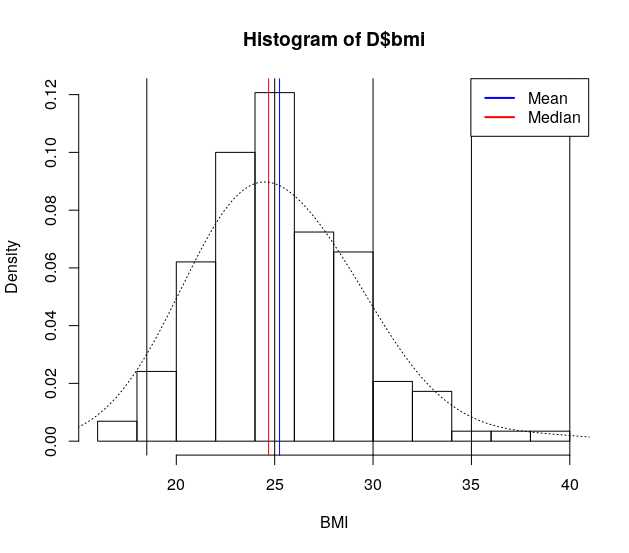
\includegraphics[scale=0.7]{Hist.png}
	\caption{Density histogram of BMI}
\end{figure}
From the histogram we can see that most of the observed BMI's lie within 20-30 $\frac{kg}{m^2}$ which are the two categories: normal weight and moderately overweight. This means that the majority of people are around normal weight or moderately overweight. If we plot the median(24.69) and mean(25.25), we see that the distribution is right skewed since the mean is to the right of the median. 
BMI scores cannot be negative since what we are getting out of the formula is $\frac{kg}{m^2}$ and a person cannot have negative weight or height. 
The standard deviation is found to be 3.83, which shows that there is some variation in the observations since we see a lot of different BMI values, with the minimum being 17.6 and the maximum being 39.5. 

\section{c) - Gender density histograms}
\begin{figure}[H]
	\centering
	\begin{minipage}{0.5\textwidth}
		\centering
		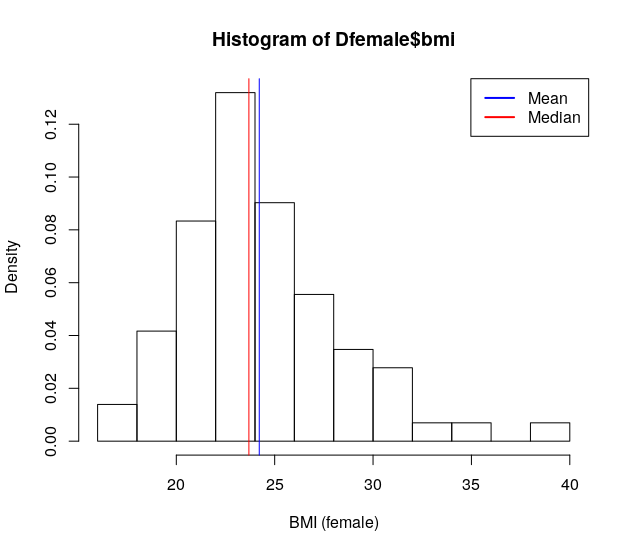
\includegraphics[width=1\textwidth]{femalehist.png}
		\caption{Histogram of female BMI scores}
	\end{minipage}\hfill
	\begin{minipage}{0.5\textwidth}
		\centering
		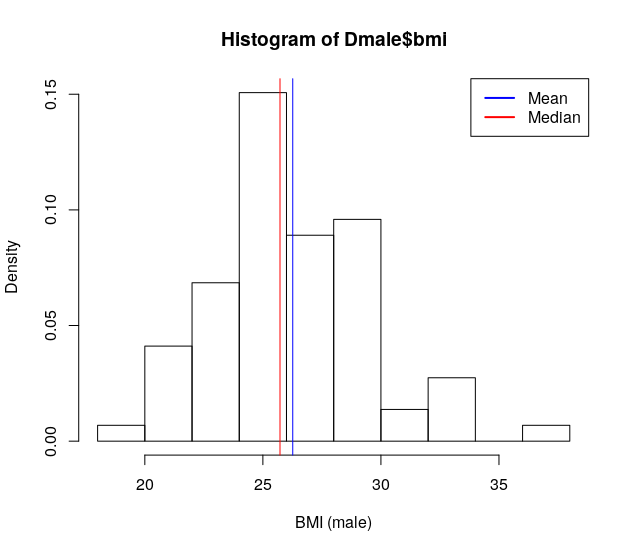
\includegraphics[width=1\textwidth]{malehist.png}
		\caption{Histogram of male BMI scores}
	\end{minipage}
\end{figure}
We can see from the figures above that both histograms are right-skewed since the mean(blue) is on the right side of the median(red) in both density histograms.
For the female BMI observations, it is seen that they are primarily distributed around 20-26 which means that most of the female weights are within the normal weight category.
If we look at the male density histogram, we see that most of the male weights are within 23-30, which shows that the men are generally a bit higher in their BMI than females. Male BMIs are generally in the normal to moderately weight categories. 

The standard deviation for the female observations is 4.1 so there is a quite a bit of variation in the values with the minimum being 17.6 and the maximum being 39.5 with the mean 24.2 and median 23.7. 
The standard deviation for the male observations is 3.3 so there is still some variation but not as much as in the female observations. The minimum is 19.8 and the maximum is 37.6 with the mean 26.3 and the median 25.7. 

Generally the male BMI scores are higher than the female BMI scores and not as spread out. 

\section{d) - Box plot}
\begin{figure}[H]
	\centering
	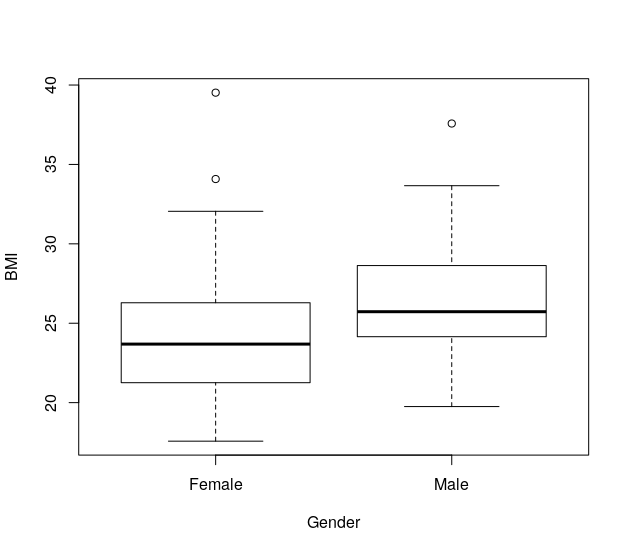
\includegraphics[scale=0.7]{boxplot.png}
	\caption{Box plot of BMI scores for each gender}
\end{figure}
From the female BMI box plot we can conclude that the distribution is right-skewed, however not by much. The male BMI box plot is much more clearly right-skewed. 
There are some differences which are the same differences as observed before; the male BMI scores are generally higher and less spread out. It is perhaps a bit more easily observed on the box plot. 
We can easily distinguish extreme outliers on the box plot as they are plotted as single points. There are two for the female observations and one for the male observations. 

\section{e) - BMI summary statistics}

\begin{table}[!h]
\centering
\caption{BMI score summary statistics table}
\label{table 1.4}
\resizebox{\textwidth}{!}{%
\begin{tabular}{llllllll}
BMI & Number of obs. & Sample mean & Sample variance & Sample std. dev. & Lower quartile & Median & Upper quartile \\
 & n & $\bar{x}$ & $s^2$ & s & $Q_1$ & $Q_2$ & $Q_3$ \\
Everyone & 145 & 25.25 & 14.69 & 3.83 & 22.59 & 24.69 & 27.64 \\
Female & 72 & 24.22 & 16.42 & 4.05 & 21.26 & 23.69 & 26.29 \\
Male & 73 & 26.27 & 11.07 & 3.33 & 24.15 & 25.73 & 28.63
\end{tabular}%
}
\end{table}
Compared to the box plot, we can see a bit more information from this table. Number of observations, variance and standard deviation are not included in the box plot. The standard deviation in particular can provide some more information about the spread of the observations.
\clearpage

\chapter[Statistical Analysis]{\\ Statistical Analysis}
\section{f) - Statistical model for BMI}
We try to plot the logarithmic-transformed BMI values as a QQ plot. The QQ plot can be used to check whether the logarithmic-transformed BMI values follow a normal distribution. 
\begin{figure}[H]
	\centering
	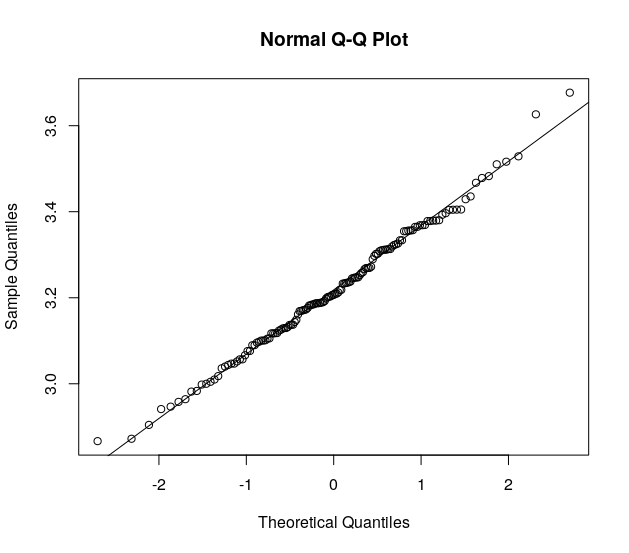
\includegraphics[scale=0.6]{qqplot1.png}
	\caption{QQ-plot normal distribution}
\end{figure}
From the above figure we can see that since the values nicely follows a straight line, the BMI follow a normal distribution.
The logarithmic mean and logarithmic standard deviation are estimated to be 3.22 and 0.15 respectively. When looking at the QQ plot we can see that these values seem to be quite accurate as the values follows a straight line (for a normal distribution) quite nicely. The mean can be seen where the theoretical quantiles = 0 and the standard deviation is how much the values deviate from the straight line. 
Since the log values follow the normal distribution line, we have validated that the log-transformed observations follow a normal distribution. Furthermore it is validated since all individual observations are independent. 
If we consider the Central Limit Theorem, we can conclude that if we had more observations the observations would follow a normal distribution better, and if we had less, it would not be as close to a normal distribution as it is. 

\section{g) - Confidence interval formula}
We insert the numbers into the formula for confidence interval: 
$$ \bar{x} \pm t_{0.975} \cdot \frac{s}{\sqrt{n}}$$
$$ 3.2176 \pm 1.9765 \cdot \frac{0.1489}{\sqrt{145}}$$
From this we get the confidence interval to be: [3.193 ; 3.242], which is correct if we check with the t.test function in r. 
Now we find the confidence interval for the median BMI scores by using the exponential function on the already calculated confidence interval. 
$$ e^{3.193} ; e^{3.242} $$
Which gives us a median BMI confidence interval [24.366 ; 25.587]

\section{h) - hypothesis test}
The significance level $\alpha$ is set to $5 \% $, the formula for the test statistics is:
$$ t_{obs} = \frac{\bar{x}-\mu_{0}}{s / \sqrt{n}} $$
$$ \frac{3.218-log(25)}{0.1489 / \sqrt{145}} = -0.0999 = t_{obs}$$
The test statistics follow a normal distribution and we have 144 degrees of freedom. 
We have already calculated the test statistics and the p-value is found to be 0.92. This is done by using the R command: P(T>x)=2(1-pt(D\$logbmi,144)). 

We hereby accept the null-hypothesis as the p-value is larger than $\alpha$.
Now we can conclude that since the null-hypothesis is accepted, we cannot deny that the average BMI score is 25, which is right on the tipping-point between the normal weight category and the overweight category. 

\section{i) - statistical models for female and male BMI}
We will assume that both male and female BMI scores are normally distributed. So we will create a QQ plot for both in order to check this assumption and validate the model. 
\begin{figure}[H]
	\centering
	\begin{minipage}{0.5\textwidth}
		\centering
		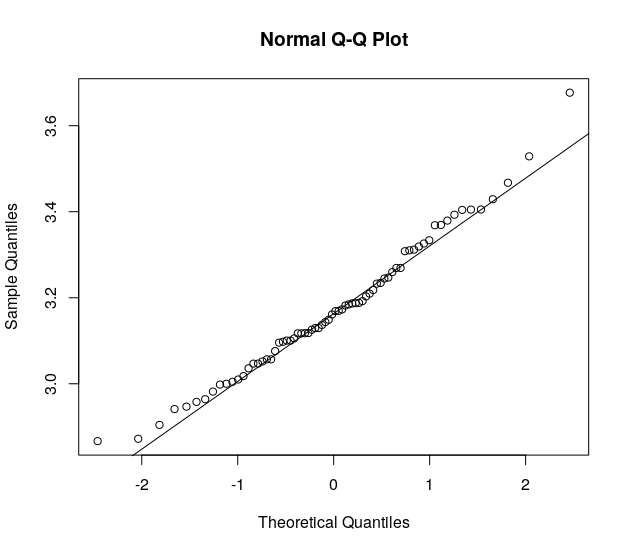
\includegraphics[width=1\textwidth]{femalelog.png}
		\caption{QQ plot of female log-transformed BMI}
	\end{minipage}\hfill
	\begin{minipage}{0.5\textwidth}
		\centering
		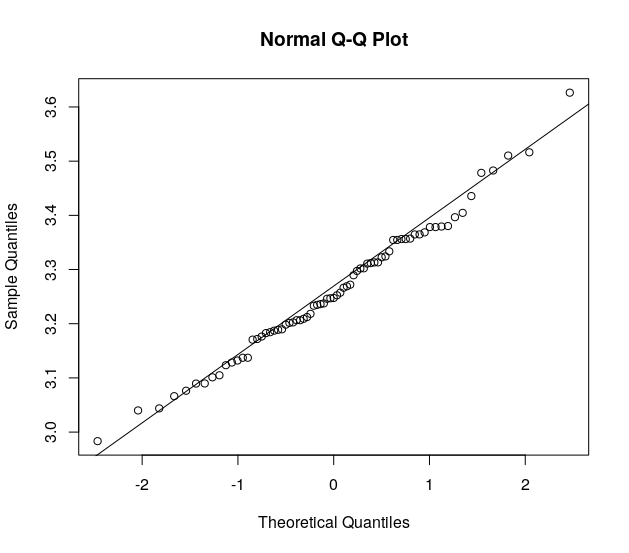
\includegraphics[width=1\textwidth]{malelog.png}
		\caption{QQ plot of male log-transformed BMI}
	\end{minipage}
\end{figure}
We can see from the QQ plots that both male and female log transformed BMI scores follow a normal distribution nicely. The mean can be estimated to 3.17 for females and 3.26 for men. The standard deviation is 0.16 for females and 0.12 for males. 
Overall we see that the male values do not vary as much as the females and the mean is a bit higher, meaning their BMI will generally be higher than the females. At least according to the data.
\section{j) - median confidence interval }
We calculate the CI with the same formula as previously used
\begin{table}[]
\centering
\caption{Calculated median BMI CI}
\label{table 2.3}
\resizebox{0.45\textwidth}{!}{%
\begin{tabular}{lll}
      & Lower bound of CI & Upper bound of CI \\
Women & 23.02             & 24.82             \\
Men   & 25.32             & 26.83            
\end{tabular}%
}
\end{table}
When compared with the results from the R code, we see that the values are the same. 
\section{k) - hypothesis test}
So with $H_0 $ being that there is no difference in male and female BMI scores. $\alpha = 5\%$. The formula for the test statistic: 
$$ t_{obs} = \frac{\bar{x}-\mu_{0}}{s / \sqrt{n}} $$
Which is calculated with the values from table \ref{table 1.4} to be -3.33. 
We find the degrees of freedom by using the formula: 
$$ v = \frac{(\frac{(s_1)^2}{n_1}+\frac{(s_2)^2)}{n_2})^2}{\frac{((s_1)^2/(n_1))^2}{n_1-1}+\frac{((s_2)^2/(n_2))^2}{n_2-1}}  $$
$$ v = \frac{(\frac{(4.05)^2}{72}+\frac{(3.33)^2)}{73})^2}{\frac{((4.05)^2/(72))^2}{71}+\frac{((3.33)^2/(73))^2}{72}} = 133.75 $$
Now the p-value is found to be 0.000392 which means that we can reject the null-hypothesis, since the p-value is much lower than $\alpha$. 
For our data it means that there is a difference between the distributions for male and female BMI scores.

\section{l) - Comment on the hypothesis test}
If we take a look at the confidence intervals in table \ref{table 2.3}. From these we could have concluded that the two score-groups are very significantly different, since the CI intervals do not overlap.

\section{m) - Correlation between BMI and weight} 
With BMI as x and weight as y, the formula for calculating correlation is then: 
$$ r = \frac{1}{n-1} \sum_{i = 1}^{n} (\frac{x_i-bar(x)}{s_x}) (\frac{y_i-bar(y)}{s_y}) = \frac{s_{xy}}{s_x \cdot s_y}$$ 
The correlation is now calculated and we get the following result. We have a strong correlation between weight and BMI, exactly 0.828. 
Now we calculate the correlation between weight, fastfood and BMI. 
We get the following correlation:
\begin{table}[H]
\centering
\caption{Correlation}
\label{table 2.4}
\resizebox{0.25\textwidth}{!}{%
\begin{tabular}{lll}
weight & 0.279    & 0.828 \\
0.279  & fastfood & 0.153 \\
0.828  & 0.153    & bmi  
\end{tabular}%
}
\end{table}

We plot the correlation: 

\begin{figure}[H]
	\centering
	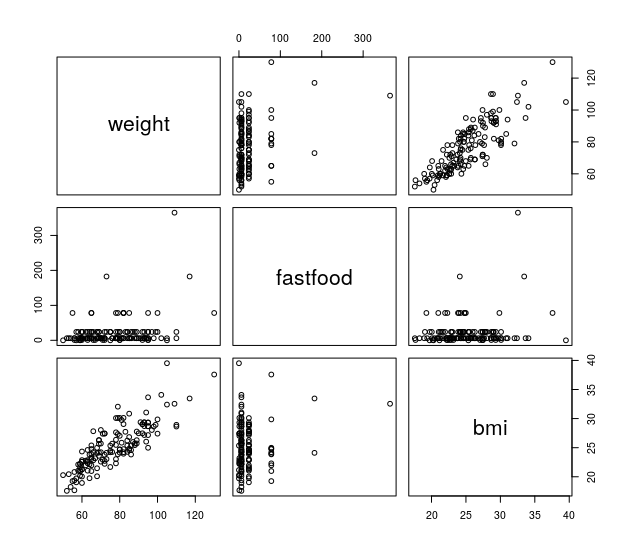
\includegraphics[scale=0.8]{scatter.png}
	\caption{Scatter plot of correlation}
\end{figure}
From the correlation values and the plot, we can see that there is only a significant correlation between weight and BMI. The other values are too low to conclude any correlation.


%----------------------------------------------------------------------------------------
%	BIBLIOGRAPHY
%----------------------------------------------------------------------------------------
%\clearpage
%\addcontentsline{toc}{chapter}{References}
%\bibliographystyle{ieeetr}
%\bibliography{/home/frederik/Documents/bibtex/SON.bib}
\end{document}
